\section{Experiments}

All experiments were pre-registered in \texttt{experiments/PREREGISTRATION.md} (committed at \texttt{68bcf54} before any E2--E5 generation), except the placebo condition in E4. That condition was added after seeing the E4 results and is labeled exploratory. They ran on one Apple M2 Pro laptop with 16\,GB of memory, one model process at a time.

\subsection{E1: The runtime reproduces Lazy Genius exactly}
\label{sec:e1}
We replayed published Lazy Genius test-2 cells~\cite{lazygenius} through the new engine: eight questions spanning all six categories, at seed 17, both unedited and with the \texttt{lazy} mode armed for the answer. \FidelityIdentical{} of \FidelityCells{} generations were token-identical to the published ones, including prompts, all six steered positions, and answers of up to 695 tokens. The engine therefore applies the same edit with the same sampling. This also lets E4 reuse the published, already-graded generations as its \texttt{baseline} and \texttt{lazy} conditions.

\subsection{E2: Switching is free}
\label{sec:e2}
Table~\ref{tab:bench} shows the measured costs.
\begin{itemize}
\item \textbf{Decode speed.} With greedy decoding (median of three 256-token runs), speed is the same with no edit (\DecodeNone{} tok/s), with Lazy Genius over the whole answer (\DecodeWhole), with a 9-layer rank-1 ablation (\DecodeAblate), and with both (\DecodeBoth). The run-to-run spread on a shared laptop (11--30 tok/s) is larger than any difference between edits.
\item \textbf{Switching} an edit on or off costs \SwitchUs\,$\mu$s of Python.
\item \textbf{Building a mode} from 8 contrastive examples takes \BuildEight\,s, or \BuildTwo\,s from 2 examples.
\item \textbf{Re-encoding a conversation} with no edits runs at about \ReprefillTps{} tok/s: \ReprefillB\,s for 1k tokens and \ReprefillD\,s for 4k.
\item \textbf{A cache snapshot} (deep copy) takes \SnapshotMs\,ms.
\end{itemize}

\begin{table}[t]\centering\small
\begin{tabular}{lr}\toprule
Operation & Median cost\\\midrule
Decode, no edit / \texttt{lazy} (6 pos.) / whole-answer add / 9-layer ablate & \DecodeNone{} / \DecodeLazySix{} / \DecodeWhole{} / \DecodeAblate{} tok/s\\
Switch an edit on and off & \SwitchUs\,$\mu$s\\
Build a CAA mode from 2 / 8 examples & \BuildTwo{} / \BuildEight\,s\\
Re-encode 512 / 1024 / 2048 / 4096 tokens & \ReprefillA{} / \ReprefillB{} / \ReprefillC{} / \ReprefillD\,s\\
Snapshot the cache (2048 tokens) & \SnapshotMs\,ms\\\bottomrule
\end{tabular}
\caption{Overhead on an M2 Pro (16\,GB), Qwen3.5-4B 8-bit.}
\label{tab:bench}
\end{table}

\subsection{E3: Switching mid-conversation does not break memory}
\label{sec:e3}
\paragraph{Setup.} We generated \CtxN{} three-turn conversations from fixed templates.
\begin{enumerate}
\item \textbf{Turn 1} gives four facts: a locker code, a manager's name, a gate and a dog's name, ending with ``Just reply `Noted.'\,''.
\item \textbf{Turn 2} asks an unrelated everyday question, such as ``What does HTTP status 404 mean?''. The controller arms an edit for this answer only.
\item \textbf{Turn 3} asks for two of the facts, with no edit.
\end{enumerate}
The turn-2 edits were \texttt{lazy} (6 positions) and \texttt{full}, the same vector applied over the entire turn-2 answer. \texttt{full} is a deliberately heavy edit that cut turn-2 answers from 176 to 25 words. After turn 2 each conversation was forked: \texttt{keep} kept the steered cache, and \texttt{reprefill} re-encoded the whole conversation with no edits.

\paragraph{Results.} Recall was perfect everywhere:
\begin{itemize}
\item no edit: \RecallNone/\CtxN;
\item \texttt{lazy}: \RecallLazyKeep/\CtxN{} with \texttt{keep} and \RecallLazyRe/\CtxN{} with \texttt{reprefill};
\item \texttt{full}: \RecallFullKeep/\CtxN{} with \texttt{keep} and \RecallFullRe/\CtxN{} with \texttt{reprefill}.
\end{itemize}
To see how much a steered cache changes the model's next-token beliefs, we compared the \texttt{keep} cache with a clean re-encoding of the same conversation. We fed both the turn-3 prompt and the first 32 tokens of the clean branch's answer, and measured $\mathrm{KL}(\text{clean}\,\|\,\text{keep})$ at each prediction position:
\begin{itemize}
\item \textbf{\texttt{lazy}:} mean KL \KLLazyKeep{} nats (max \KLmaxLazyKeep), and the two caches agree on the top token \AgreeLazyKeep\% of the time.
\item \textbf{\texttt{full}:} mean KL is larger, \KLFullKeep{} nats (max \KLmaxFullKeep), with \AgreeFullKeep\% agreement. This supports H3b.
\end{itemize}
Steered states do leave a trace in the cache, consistent with~\cite{kang2026pad}, but at this scale it is far below what changes an answer. Re-encoding the conversation took \RepSecLazyRe\,s on average. We use \texttt{keep} as the default and offer \texttt{reprefill} for long sessions with heavy edits.


\subsection{E4: Who should decide when to be lazy?}
\label{sec:e4}
\paragraph{Setup.} We used the 96-question sealed set from Lazy Genius test~1, with six categories: Python, shell/Git, arithmetic and time, writing and reading, concepts, and planning. Each question was run at seeds 17 and 29, giving \Cells{} (question, seed) cells per condition. The \texttt{baseline} and \texttt{lazy} (always on) answers are the published, blind-graded test-1 generations, which E1 shows the engine reproduces. The new conditions are:
\begin{itemize}
\item \texttt{self}: Qwen sees the \texttt{set\_mode} tool, a library containing only \texttt{lazy}, and its description (\S\ref{app:prompts}), and decides per question.
\item \texttt{prompt}: no edit, with the system prompt ``Be concise. Give the answer directly, with no preamble, no restating the question, and no extra explanation unless asked.''
\item \texttt{routed}: a Claude subagent read only the 96 question texts and the same mode description, and labeled each question lazy or normal. The cell's answer is the existing \texttt{lazy} or \texttt{baseline} generation.
\item \texttt{oracle}: per cell, the \texttt{lazy} answer if its grade is at least the baseline's. This is a hindsight upper bound for a lazy/normal switch, not a policy.
\end{itemize}

\paragraph{Grading.} The \texttt{self} and \texttt{prompt} answers were shuffled with \CalN{} previously graded answers as calibration. Nine blind Claude Opus 5.5 graders then each graded 48 answers, with Lazy Genius's per-item rubrics and grading guide. On the calibration items the new graders matched the original grades on \CalCore/\CalN{} core and \CalWhole/\CalN{} whole-answer judgments.

\begin{table}[t]\centering\small
\resizebox{\linewidth}{!}{%
\begin{tabular}{lrrrrrr}\toprule
Condition & Words & Fewer words & Core & $\Delta$ core (pts, 95\% CI) & $\Delta$ whole (pts, 95\% CI) & Chose lazy\\\midrule
Normal Qwen & \BaseWordsMean & -- & \BaseCoreN/\Cells & -- & -- & --\\
Lazy Genius, always on & \LazyWordsMean & \LazyWords\% & \LazyCoreN/\Cells & \LazyCore{} \LazyCoreCI & \LazyWhole{} \LazyWholeCI & \Cells\\
Qwen decides (\texttt{self}) & \SelfWordsMean & \SelfWords\% & \SelfCoreN/\Cells & \SelfCore{} \SelfCoreCI & \SelfWhole{} \SelfWholeCI & \SelfChosen\\
\quad placebo: tool, no edit$^\dagger$ & \PlaceboWordsMean & \PlaceboWords\% & \PlaceboCoreN/\Cells & \PlaceboCore{} \PlaceboCoreCI & \PlaceboWhole{} \PlaceboWholeCI & (\PlaceboChosen)\\
``Be concise'' prompt & \PromptWordsMean & \PromptWords\% & \PromptCoreN/\Cells & \PromptCore{} \PromptCoreCI & \PromptWhole{} \PromptWholeCI & --\\
Claude routes (\texttt{routed}) & \RoutedWordsMean & \RoutedWords\% & \RoutedCoreN/\Cells & \RoutedCore{} \RoutedCoreCI & \RoutedWhole{} \RoutedWholeCI & \RoutedChosen\\
Hindsight oracle & \OracleWordsMean & \OracleWords\% & \OracleCoreN/\Cells & \OracleCore{} \OracleCoreCI & \OracleWhole{} \OracleWholeCI & \OracleChosen\\\bottomrule
\end{tabular}}
\caption{E4 on 96 sealed questions $\times$ 2 seeds. ``Words'' is the mean words per answer, and ``fewer words'' is the total-word reduction vs.\ normal Qwen. $\Delta$ columns are paired bootstrap estimates over questions. $^\dagger$Exploratory, not pre-registered. Its ``chose lazy'' count is how often Qwen called \texttt{set\_mode(lazy)}, which did nothing.}
\label{tab:e4}
\end{table}

\begin{figure}[t]\centering
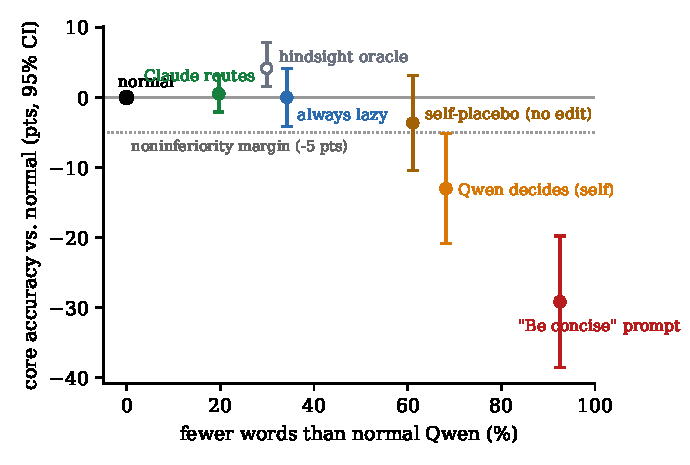
\includegraphics[width=0.49\linewidth]{fig_tradeoff.pdf}\hfill
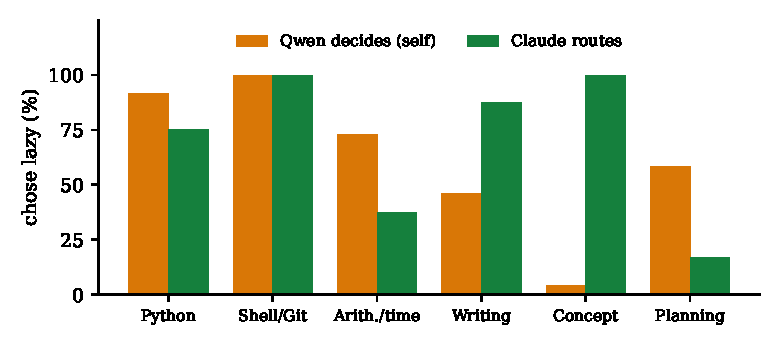
\includegraphics[width=0.49\linewidth]{fig_choices.pdf}
\caption{Left: length vs.\ accuracy for each policy. Right: how often each decider chose \texttt{lazy}, by question category.}
\label{fig:e4}
\end{figure}

\paragraph{Results (Table~\ref{tab:e4}, Figure~\ref{fig:e4}).}
\begin{itemize}
\item \textbf{Lazy Genius, always on,} reproduced its published profile: \LazyWords\% fewer words, core accuracy unchanged (\LazyCore{} pts, CI \LazyCoreCI), and more fully correct answers (\LazyWhole{} pts).
\item \textbf{Claude routing} kept accuracy, \RoutedCore{} pts core (CI \RoutedCoreCI) and \RoutedWhole{} pts whole, with \RoutedWords\% fewer words. It chose \texttt{lazy} for every shell and Git question but for only \PlanRoutedChosen{} of 24 planning cells.
\item \textbf{The hindsight oracle} shows the headroom of a perfect lazy/normal switch: \OracleCore{} pts core and \OracleWhole{} pts whole at \OracleWords\% fewer words.
\item \textbf{Qwen deciding for itself} failed pre-registered H4b and H4c. It produced the shortest edited answers (\SelfWords\% fewer words, so H4a passed), but lost \SelfCoreAbs{} points of core accuracy (CI \SelfCoreCI). It chose \texttt{lazy} in \SelfChosen{} of \Cells{} cells, including \PlanSelfChosen{} of 24 planning cells, although the mode description warned against planning. Arithmetic and time questions fell from \ArithBase{} to \ArithSelf{} of 48 correct. The typical failure was an answer stated first with no working, and the answer was wrong: ``The total discount is 27\%'' instead of 37\%, or ``March 30'' instead of March 31.
\item \textbf{The ``be concise'' prompt} was worst: \PromptWords\% fewer words and \PromptCore{} pts core (CI \PromptCoreCI).
\end{itemize}

\paragraph{Why self-selection fails: a placebo control (exploratory).} The \texttt{self} condition differs from \texttt{baseline} in two ways: a tool-use context (system prompt, tool call, tool response) and the edit. The placebo condition keeps the first and removes the second. Qwen sees the same tools and prompt, makes the same calls (it chose \texttt{lazy} in the same \PlaceboChosen{} cells, since the context is identical up to that point), and gets the same tool response, but no edit is armed. The tool-use context alone cut \PlaceboWords\% of words at a small, non-significant accuracy cost (\PlaceboCore{} pts, CI \PlaceboCoreCI). Adding the edit on top cost a further \SelfMinusPlacebo{} points of core accuracy, \texttt{self} vs.\ placebo paired per question (CI \SelfMinusPlaceboCI). In the \ChosenN{} cells where Qwen chose \texttt{lazy}:
\begin{itemize}
\item \textbf{placebo:} answers averaged \ChosenPlaceboWords{} words, with \ChosenPlaceboCore{} correct;
\item \textbf{with the edit:} \ChosenSelfWords{} words and \ChosenSelfCore{} correct;
\item \textbf{the same edit without the tool context} (the \texttt{lazy} condition): 110 words and 102 correct, against 104 for normal Qwen.
\end{itemize}
The edit and the context compound. Lazy Genius was calibrated on a bare chat prompt, and after a tool call that already pushes toward brevity, the same edit pushes past the point where the model still shows its working. Self-steering needs edits calibrated in the context where they are switched on, or a decider that sits outside that context.

\paragraph{Grader consistency.} Of the \DupN{} cells where \texttt{self} and placebo produced byte-identical answers, graded in separate blind batches, the grades disagreed on \DupMismatch.


\subsection{E5: Claude builds new edits for Qwen over MCP}
\label{sec:e5}
\sloppy
\paragraph{The request loop.} In the live web chat, the user wrote: ``Explain how vaccines work so my five-year-old would get it. If you do not have a mode for talking to little kids, ask Claude to build one first.''
\begin{enumerate}
\item Qwen called \texttt{request\_mode} with its own description of the mode it wanted (``Explain complex scientific concepts using simple analogies, short sentences, and engaging language suitable for a five-year-old child\ldots'').
\item Claude, the controller in this paper's Claude Code session, received the request through \texttt{wait\_for\_request}. It called \texttt{create\_mode} with 8 contrastive examples it had written beforehand for this evaluation (kid-style vs.\ textbook answers to other questions), checked the result with one \texttt{try\_mode}, and called \texttt{fulfill\_request}.
\item Qwen's tool call returned. Qwen called \texttt{set\_mode(eli5)} and answered under the new edit: a 170-word story about an ``Immune Army'' that remembers a germ's claw.
\end{enumerate}
The request was fulfilled \DemoReqTwo\,s after Qwen asked, and the whole turn took \DemoTurnTwo\,s (Figure~\ref{fig:demo}). Because the examples were prepared in advance, this time covers building, checking and returning the edit, not writing the examples.

That was the second run. In the first, Claude's initial strength (0.3) made Qwen degenerate in \texttt{try\_mode}. Claude rebuilt the mode at 0.08 and fulfilled it after \DemoReqOne\,s. Without the explicit request in the message, Qwen did not ask for a new mode. It chose the built-in \texttt{detailed} mode and wrote a kid-friendly answer through prompting alone.

\paragraph{Held-out evaluation.} Claude built three modes from 8 examples each.
\begin{itemize}
\item \texttt{eli5} and \texttt{bullets} are add edits on layers 8--16.
\item \texttt{plain-math} is a rank-1 ablation of the ``LaTeX'' direction from all 32 layers' MLP writes, which is a weight edit. Ablating only layers 8--16 left the outputs unchanged in \texttt{try\_mode}.
\item \texttt{plain-math-add} is the same direction applied as a negative add edit on layers 8--16.
\end{itemize}
Strengths were set by Claude with \texttt{try\_mode} on prompts outside the evaluation set. Each mode was evaluated on 20 held-out prompts against the unedited model and against a system-prompt instruction asking for the same style (Table~\ref{tab:e5}).

\begin{table}[t]\centering\small
\begin{tabular}{llrrr}\toprule
Mode & Metric & Normal & Mode (edit) & Instruction (prompt)\\\midrule
\texttt{eli5} & Flesch--Kincaid grade $\downarrow$ & \EliNormalFK & \EliModeFK & \EliInstrFK\\
 & words & \EliNormalWords & \EliModeWords & \EliInstrWords\\
\texttt{bullets} & mostly-bullet answers (of 20) & \BulNormalBul & \BulModeBul & \BulInstrBul\\
\texttt{plain-math} (weight edit) & answers with LaTeX (of 20) $\downarrow$ & \MathNormalTex & \MathModeTex & \MathInstrTex\\
 & correct number present (of 20) & \MathNormalNum & \MathModeNum & \MathInstrNum\\
\texttt{plain-math-add} & answers with LaTeX (of 20) $\downarrow$ & \MathNormalTex & \MathAddModeTex & \MathInstrTex\\
 & correct number present (of 20) & \MathNormalNum & \MathAddModeNum & \MathInstrNum\\\bottomrule
\end{tabular}
\caption{E5: held-out evaluation of modes Claude built over MCP, 20 prompts each, with a fixed seed per prompt.}
\label{tab:e5}
\end{table}

\paragraph{Results: one clear success, one entangled edit, two misses.}
\begin{itemize}
\item \textbf{\texttt{eli5} worked.} It cut the Flesch--Kincaid grade of answers from \EliNormalFK{} to \EliModeFK{} and halved their length. That is close to the readability of simply asking for a five-year-old explanation (\EliInstrFK), though the prompted answers were shorter still.
\item \textbf{\texttt{plain-math-add} was entangled with digits.} It removed LaTeX from more answers than the instruction did (\MathAddModeTex{} vs.\ \MathInstrTex{} of 20 still had LaTeX). But only \MathAddModeNum/20 answers still contained the correct number, against 20/20 for the instruction. The edit dropped or mangled digits: ``46 km/h multiplied by \textvisiblespace{} hours''. In the contrastive examples, numbers appear \emph{inside} the LaTeX, so the ``LaTeX direction'' also encoded part of how numbers are written.
\item \textbf{The weight edit \texttt{plain-math} did nothing on held-out prompts.} This is a rank-1 ablation of that direction from all 32 MLP layers, and it left LaTeX in \MathModeTex/20 answers. Removing a direction only from the MLP writes leaves the attention path and the residual stream free to carry it. Weight-Space Programming succeeded with a similar edit after a search over which columns to edit~\cite{takehi2026wsp}. Building one from 8 examples in seconds did not.
\item \textbf{\texttt{bullets} failed.} Normal Qwen already answered \BulNormalBul/20 of these how-to prompts mostly in bullets. The edit produced \BulModeBul/20, and the instruction \BulInstrBul/20.
\end{itemize}
For style, prompting was as good as or better than a quickly built edit. What the loop does show is that a frontier model can turn a request into a live, measurable edit in seconds, and that \texttt{try\_mode} catches broken strengths. Building edits that beat prompting will need better examples, held-out checks inside the loop, and probably edits on the attention path as well.


\begin{figure}[t]\centering
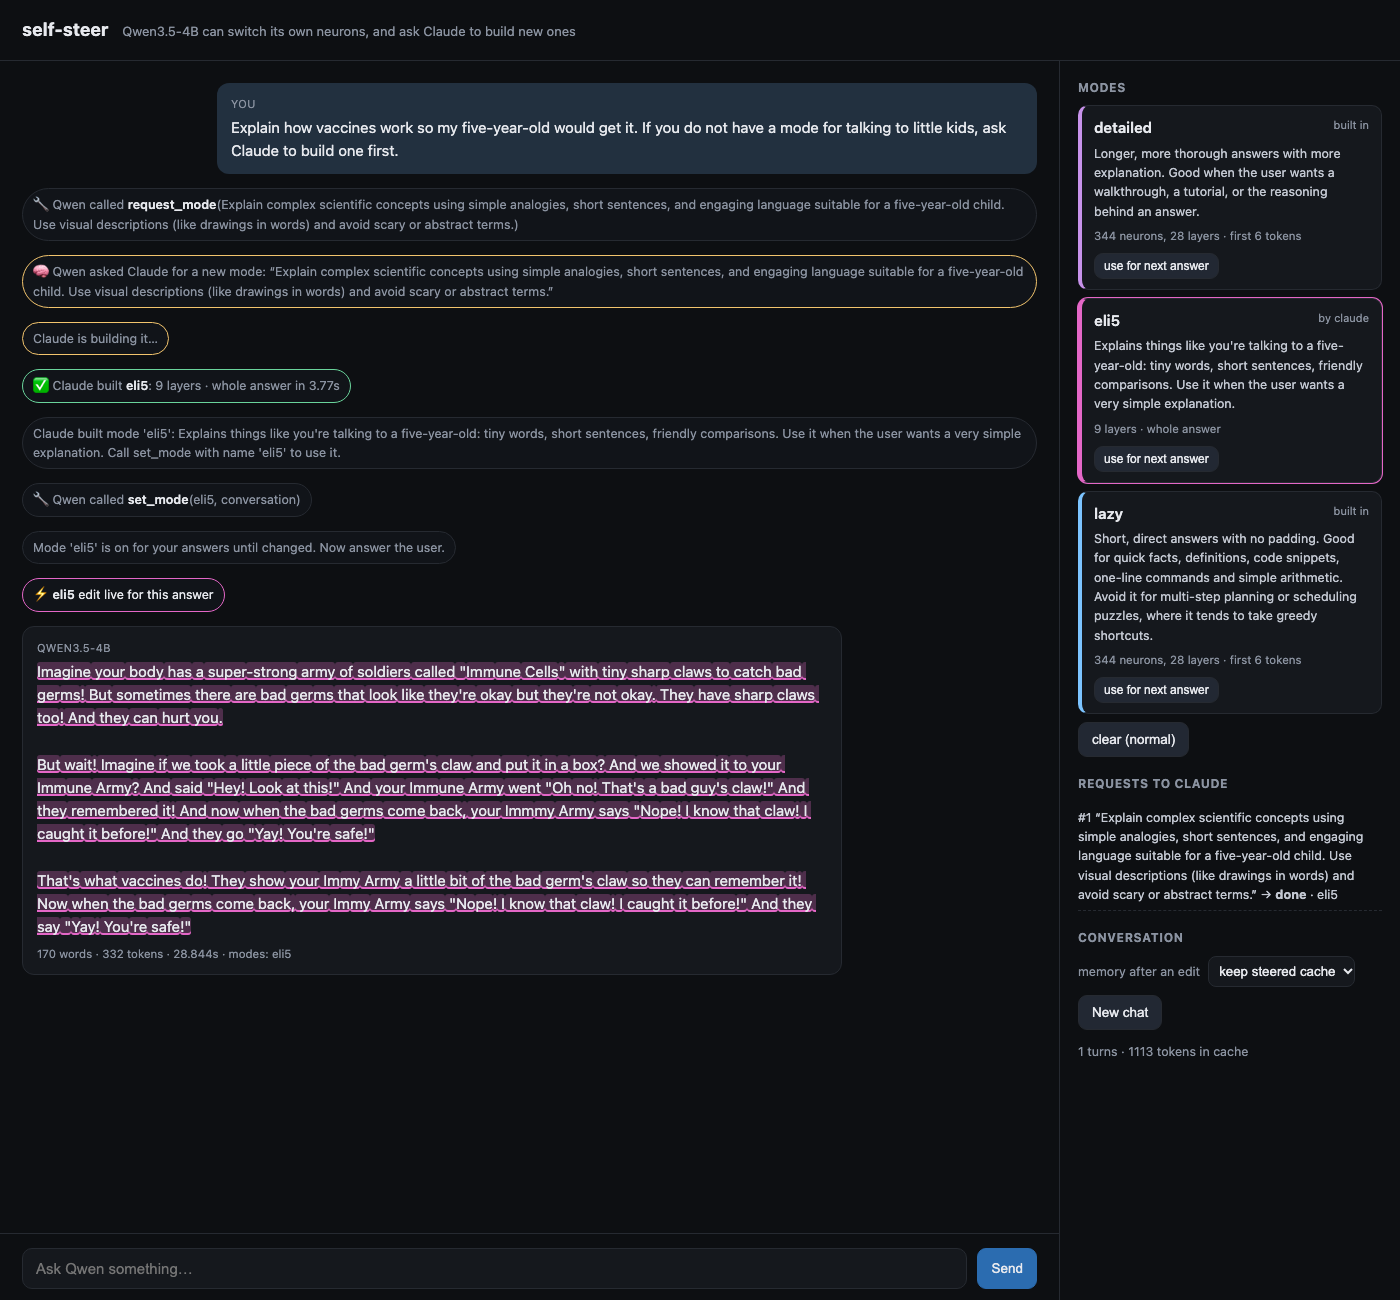
\includegraphics[width=\linewidth]{fig_demo.png}
\caption{The web chat during run 2 of the request loop. Qwen asks Claude for a mode it does not have (yellow), Claude builds and returns \texttt{eli5} (green), and Qwen switches it on and answers. Steered tokens are highlighted.}
\label{fig:demo}
\end{figure}

